\documentclass{article}
\usepackage{tikz}
\usetikzlibrary{arrows, snakes, backgrounds}
\begin{document}
\begin{tikzpicture}
\draw (0,0) -- (1,1);
\end{tikzpicture}
\begin{tikzpicture}
\path (0,1) node [shape=circle, draw]{}
	  (0,2) node [shape=circle, draw]{}
	  (0,0) node [shape=circle, draw]{}
	  (1,1) node [shape=rectangle, draw]{}
	  (-1,1) node [shape=rectangle, draw]{};
\end{tikzpicture}
\begin{tikzpicture}
\path  node at (0,1) [shape=circle, draw]{}
	   node at (0,2) [shape=circle, draw]{}
	   node at (0,0) [shape=circle, draw]{}
	   node at (1,1) [shape=rectangle, draw]{}
	   node at (-1,1) [shape=rectangle, draw]{};
\end{tikzpicture}
\tikzstyle{place} = [circle, draw = blue!50, fill=blue!20, thick,inner sep =0pt, minimum size = 6mm]
\tikzstyle{transition} = [rectangle, draw = black!50, fill= black!20, thick,inner sep = 0pt, minimum size = 4mm]
\begin{tikzpicture}[inner sep=2mm]
\node at (0,2) [place] {};
\node at (0,1) [place] {};
\node at (0,0) [place] {};
\node at (1,1) [transition] {};
\node at (-1,1) [transition] {};
\end{tikzpicture}
\begin{tikzpicture}
\node[place] (waiting 1)       at (0,2) {};
\node[place] (critical 1)	   at (0,1) {};
\node[place] (semaphore)	   at (0,0) {};
\node[transition] (leave critical) at (1,1) {};
\node[transition] (enter critical) at (-1,1) {};
\end{tikzpicture}
\begin{tikzpicture}
\node[place] (waiting)             {};
\node[place] (critical)  [below of =waiting] {};
\node[place] (semaphore) [below of =critical] {};
\node[transition] (leave critical) [right of = critical] {};
\node[transition] (enter critical) [left of = critical] {};

\node [red,above] at (semaphore.north) {$ s\leq 3$};
\end{tikzpicture}
\begin{tikzpicture}
\tikzstyle{every label} = [red]
\node[place] (waiting)             {};
\node[place] (critical)  [below of =waiting] {};
\node[place] (semaphore) [below of =critical,
						  label=above:$s\leq 3$] {};
\node[transition] (leave critical) [right of = critical] {};
\node[transition] (enter critical) [left of = critical] {};
%\draw [->] (critical.west) -- (enter critical.east);
\draw [->] (enter critical.east) -- (critical.west);
\draw [->] (waiting.west) .. controls + (left:5mm) and + (up:5mm)
						  .. (enter critical.north);
\end{tikzpicture}
\begin{tikzpicture}
\tikzstyle{every label} = [red]
\node[place] (waiting)             {};
\node[place] (critical)  [below of =waiting] {};
\node[place] (semaphore) [below of =critical,
						  label=above:$s\leq 3$] {};
\node[transition] (leave critical) [right of = critical] {};
\node[transition] (enter critical) [left of = critical] {};
%\draw [->] (critical.west) -- (enter critical.east);
\draw [->] (enter critical) -- (critical);
\draw [->] (waiting) .. controls + (left:8mm) and + (up:8mm)
						  .. (enter critical);
\end{tikzpicture}
\begin{tikzpicture}
\tikzstyle{every label} = [red]
\node[place] (waiting)             {};
\node[place] (critical)  [below of =waiting] {};
\node[place] (semaphore) [below of =critical,
						  label=above:$s\leq 3$] {};
\node[transition] (leave critical) [right of = critical] {};
\node[transition] (enter critical) [left of = critical] {};
%\draw [->] (critical.west) -- (enter critical.east);
\draw [->] (enter critical) to  (critical);
\draw [->] (waiting) to [out=180, in=90] (enter critical);

\end{tikzpicture}
\begin{tikzpicture}
\tikzstyle{every label} = [red]
\node[place] (waiting)             {};
\node[place] (critical)  [below of =waiting] {};
\node[place] (semaphore) [below of =critical,
						  label=above:$s\leq 3$] {};
\node[transition] (leave critical) [right of = critical] {};
\node[transition] (enter critical) [left of = critical] {};
%\draw [->] (critical.west) -- (enter critical.east);
\draw [->] (enter critical) to  (critical);
\draw [->] (waiting) to [bend right=45] (enter critical);
\draw [->] (enter critical) to [bend right=45] (semaphore);

\end{tikzpicture}
\begin{tikzpicture}
\tikzstyle{every label} = [red]
\node[place] (waiting)             {};
\node[place] (critical)  [below of =waiting] {};
\node[place] (semaphore) [below of =critical,
						  label=above:$s\leq 3$] {};
\node[transition] (leave critical) [right of = critical] {};
\node[transition] (enter critical) [left of = critical] {}
%\draw [->] (critical.west) -- (enter critical.east);
edge [->]                (critical)
edge [<-, bend left=45]  (waiting)
edge [->, bend right=45] (semaphore);		
\end{tikzpicture}
\tikz  \node [circle, draw, label=60:$60^\circ$, label=below:$-90^\circ$]{my circle};
\tikzstyle{pre} = [<-, shorten <= 1pt, >=stealth',semithick]
\tikzstyle{post}= [->, shorten >= 1pt, >=stealth', semithick]
\begin{tikzpicture}[bend angle=45]
\node[place]    (waiting)       {};
\node[place]    (critical)    [below of=waiting] {};
\node[place]    (semaphore)   [below of=critical] {};
\node[transition] (leave cirtical) [right of=critical] {}
edge [pre] (critical)
edge [post, bend right] node[auto,swap] {2} (waiting)
edge [pre,bend left] (semaphore);
\node[transition] (enter critical) [left of=critical] {}
edge [post] (critical)
edge [pre ,bend left] (waiting)
edge [post ,bend right] (semaphore);
\end{tikzpicture}
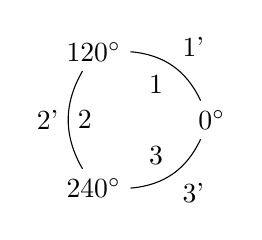
\begin{tikzpicture}[auto, bend right]
\node (a) at (0:1) {$0^\circ$};
\node (b) at (120:1) {$120^\circ$};
\node (c) at (240:1) {$240^\circ$};
\draw (a) to node{1} node [swap] {1'} (b)
	  (b) to node{2} node [swap] {2'} (c)
	  (c) to node{3} node [swap] {3'} (a);
\end{tikzpicture}
\end{document}

